%%%%%%%%%%%%%%%%%%%%%%%%%%%%%%%%%%%%%%%%%
% University/School Laboratory Report
% LaTeX Template
% Version 3.0 (4/2/13)
%
% This template has been downloaded from:
% http://www.LaTeXTemplates.com
%
% Original author:
% Linux and Unix Users Group at Virginia Tech Wiki 
% (https://vtluug.org/wiki/Example_LaTeX_chem_lab_report)
%
% License:
% CC BY-NC-SA 3.0 (http://creativecommons.org/licenses/by-nc-sa/3.0/)
%
%%%%%%%%%%%%%%%%%%%%%%%%%%%%%%%%%%%%%%%%%

%----------------------------------------------------------------------------------------
%	PACKAGES AND DOCUMENT CONFIGURATIONS
%----------------------------------------------------------------------------------------

\documentclass{article}
\usepackage{amssymb, amsmath}
\usepackage{url}
\usepackage{graphicx}
\usepackage{courier}
%\usepackage{times} % Uncomment to use the Times New Roman font

%----------------------------------------------------------------------------------------
%	DOCUMENT INFORMATION
%----------------------------------------------------------------------------------------

\title{Parallel Memory Allocation \\ A Scalable Solution \\ CSC469} % Title

\date{\today} % Date for the report

\begin{document}

\maketitle % Insert the title, author and date

\begin{center}
\begin{tabular}{l r}
Partners: & Daniel Bloemendal \\ % Partner names
& Simon Scott \\
Instructor: & Professor Angela Demke Brown % Instructor/supervisor
\end{tabular}
\end{center}

% If you wish to include an abstract, uncomment the lines below
% \begin{abstract}
% Abstract text
% \end{abstract}

%----------------------------------------------------------------------------------------
%	SECTION 1
%----------------------------------------------------------------------------------------

\section{Motivation}

\indent \indent To create a scalable parallel memory allocator with higher throughput and lower fragmentation than sequential allocators which maintains coherency.  Ideally, our allocator will also be as as good or better than the standard c malloc in these respects.


\section{Hoard Implementation}

\indent \indent We choose to implement the Hoard Memory Allocator based on both its historical significance and its utilization in modern Operating Systems.  We use a global heap, and a CPU scaling factor which can be experimentally set to determine a number of per CPU heaps to initilize.  Threads are assigned to run on specific per CPU heaps.  
\\
\indent We will use more heaps along with a more advanced hashing function in an attempt to prevent assignments of concurrent threads assigned to the same CPU.  Memory is managed in standard sized Superblocks to avoid false sharing, and we choose the system pagesize as the size for our Superblock.
\\
\indent By experimenting with the values that affect Hoards performance, we hope to further optimize our initial design.
\\
\newpage
\noindent
\textbf{Blowup}
\\
\indent  Utilizing an \textit{emptyness threshold} which can be experimentally set, we divide the Superblocks in a specific per processor heap by \textit{fullness groups}.  When a heap drops below the emptyness threshold \textit(f), and there are more than \textit(K) Superblocks worth of free memory on the heap, we transfer a superblock that is at least \textit(f) empty from the appropriate \textit{fullnes bin} back to the Global heap of free Superblocks.  By implementing this threshold, the invarient that Berger et. al. used in their experiments in their canonical paper holds (Berger et. el.).  Namely when we remove a superblock we reduce the amount of memory in use \textit{ui} by at most (1-\textit{emptyness threshold}), but we reduce the amount of memory allocated by Hoard from the Operating System \textit{ai} by \textit{S} the size of a superblock.   Maintaining this invarient bounds blowup to a constant factor (Berger et. el.).  
\\
\\
\textbf{Locality}
\\
\indent Allocated memory if requested from the highest \textit{fullness groups} first.  Fullness groups are also maintained in order of most recently freed\textit{(move to front heuristic)}.  Blocks that are reallocated are thus likley to still be in a Superblock already in memory.  Free blocks are in LIFO, so we are also liklet to use a block that is already in the cache.
\\
\\
\textbf{Fragmentation}
\\
\indent Inside Superblocks.  Superblocks keep their blocks within \textit{size classes}.  Size classes are powers of \textit{b} (where \textit{b} $>$ 1), and limit internal fragmentation to a factor of \textit{b} (Berger et. el., p.2). \textit{b} can be experimentally set.  
\\
\indent Outside Superblocks.  Superblocks are not returned to the Operating System, they are \textit{recycled} for use by any size class.
\\
\\
\textbf{False Sharing}
\\
\indent Hoard utilizes Superblocks and multiplle heaps to avoid most active and passive false sharing.  Although when the \textit{emptyness threshold} is reached and a Superblock is returned to the Global heap there is then the possibility of false sharing, Berger et. al. find in practice the returned Superblocks are mainly completley empty (Berger et. el., p.3).

\newpage

\section{Structures}

\textbf{Superblock}
\texttt{
\\
struct SUPERBLOCK\_T \{
\\
\indent   heap\_t* heap;
\\
\indent   uint8\_t group;
\\
\indent    int size\_class;
\\
\indent    size\_t block\_size;
\\
\indent    size\_t block\_count;
\\
\indent    size\_t block\_used;
\\
\indent    blockptr\_t next\_block;
\\
\indent    blockptr\_t next\_free;
\\
\indent    superblock\_t\* prev;
\\
\indent    superblock\_t\* next;
\\
\} \_\_attribute\_\_((aligned(ARCH\_CACHE\_ALIGNMENT)));
}
\\
\\
\\
\\
\noindent \textbf{Heap}
\\
\texttt{struct HEAP\_T \{
\\
\indent    int index;
\\
\indent    size\_t mem\_used;
\\
 \indent   size\_t mem\_allocated;
\\
 \indent   superblock\_t\* bins[ALLOC\_HOARD\_FULLNESS\_GROUPS];
\\
\};}
\\
\\
\\
\\
\noindent \textbf{Heap Table}
\\
\texttt{
struct CONTEXT\_T \{
\\
\indent    pthread\_mutex\_t lock;
\\
\indent    void\* blocks\_base;
\\
\indent    int heap\_count;
\\
 \indent   heap\_t heap\_table[1];
\\
\};}


\newpage
\noindent
\section{Results}
\textbf{Parameters}
\\
\\
\#define ALLOC\_HOARD\_FULLNESS\_GROUPS 4
\\
\#define ALLOC\_HOARD\_SIZE\_CLASS\_BASE 2
\\
\#define ALLOC\_HOARD\_SIZE\_CLASS\_MIN 2
\\
\#define ALLOC\_HOARD\_HEAP\_CPU\_FACTOR 1
\\
\\
\textbf{Speed}
\\
\indent Initial results show that we are considerabally better than the sequential allocators both in terms of throughput and fragmentation.
\\
\\
Results of Larson test Submit:
\\
\texttt{
greywolf:~/469/CSC469/A2/benchmarks/larson\$  ./larson-submit $<$ Input/small-6-threads
\\
Multi-threaded test driver 
\\
C version (malloc and free)
\\
runtime (sec): chunk size (min,max): threads (min, max):   chunks/thread:  no of rounds:   random seed:    
\\
thread stopping.
\\
thread stopping.
\\
thread stopping.
\\
thread stopping.
\\
area 0: 2393476 allocs, 24 threads
\\
area 1: 4054185 allocs, 41 threads
\\
area 2: 1847337 allocs, 19 threads
\\
area 3: 5058954 allocs, 51 threads
\\
area 4: 3365051 allocs, 34 threads
\\
area 5: 3933946 allocs, 40 threads
\\
Throughput =  1375508 operations per second.
\\
Memory used = 3586047 bytes, required 1440000, ratio 2.490310
\\
thread stopping.
\\
thread stopping.
\\
Done sleeping...}
\\
\\
Results of Larson test kheapt:
\\
\texttt{
greywolf:~/469/CSC469/A2/benchmarks/larson\$  ./larson-kheap $<$ Input/small-6-threads
\\
Multi-threaded test driver 
\\
C version (malloc and free)
\\
runtime (sec): chunk size (min,max): threads (min, max):   chunks/thread:  no of rounds:   random seed:
\\    
thread stopping.
\\
thread stopping.
\\
thread stopping.
\\
thread stopping.
\\
thread stopping.
\\
thread stopping.
\\
area 0: 92374 allocs, 1 threads
\\
area 1: 108222 allocs, 2 threads
\\
area 2: 59728 allocs, 1 threads
\\
area 3: 100001 allocs, 2 threads
\\
area 4: 57503 allocs, 1 threads
\\
area 5: 35419 allocs, 1 threads
\\
Throughput =    30192 operations per second.
\\
Memory used = 25997311 bytes, required 1440000, ratio 18.053688
\\
Done sleeping...
}
\\
\\
\begin{figure}[!p]
\centering
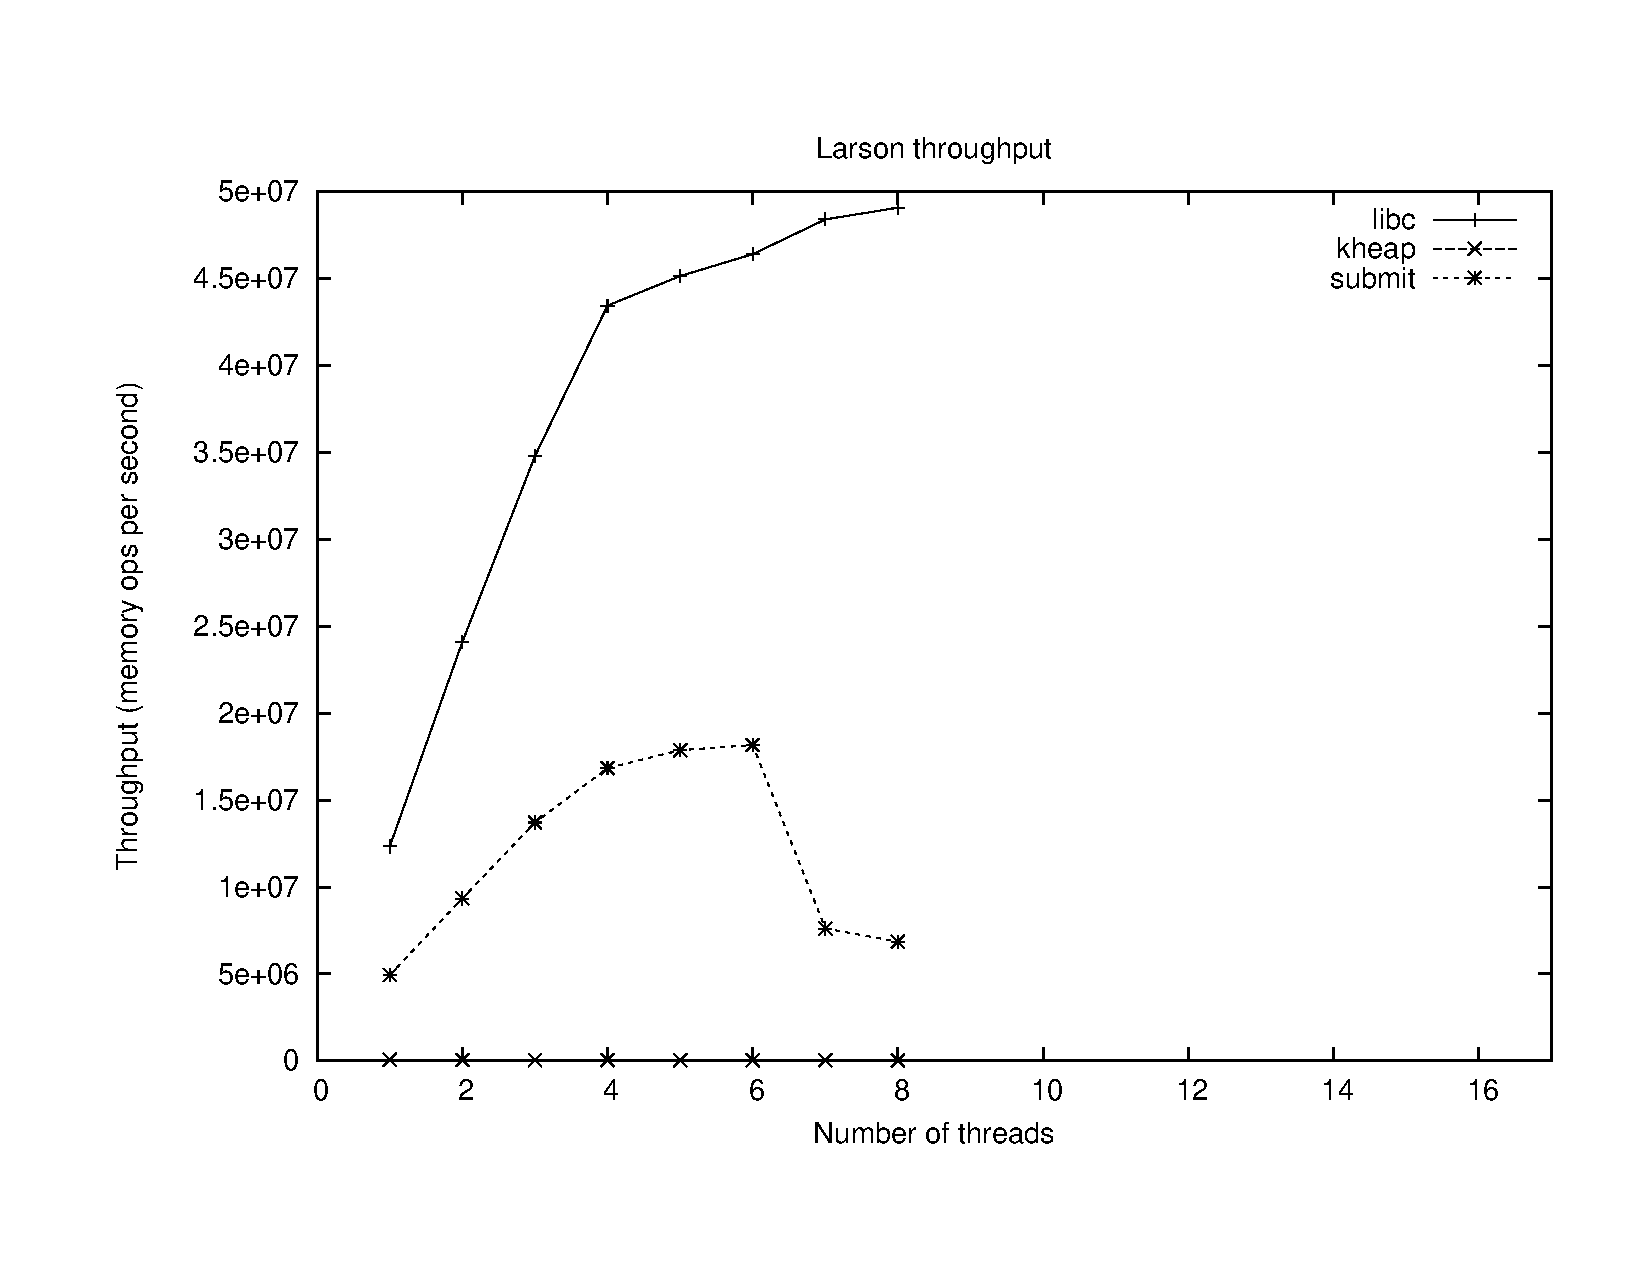
\includegraphics[width=10cm]{larson.pdf}
\caption{Larson}
\label{Larson}
\end{figure}
\\
\begin{figure}[!p]
\centering
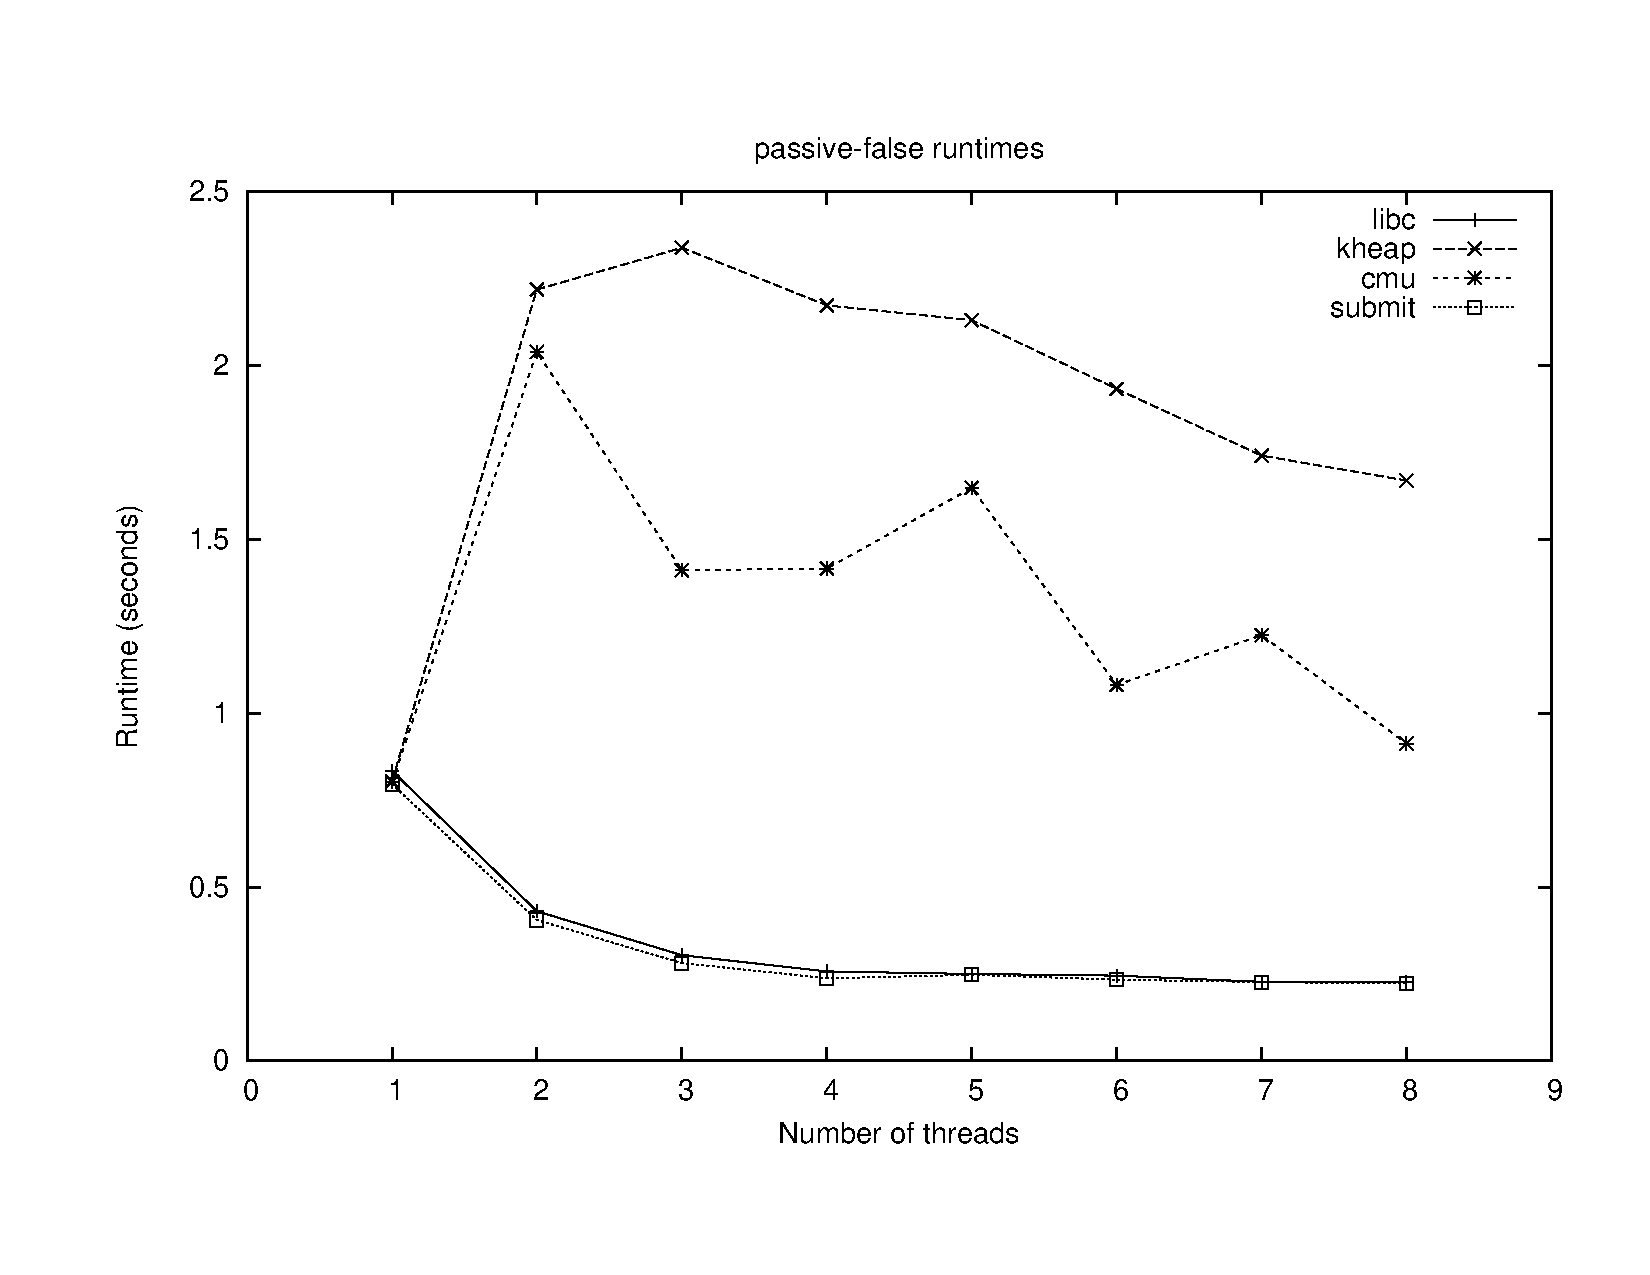
\includegraphics[width=10cm]{cache-scratch.pdf}
\caption{Cache-scratch}
\label{Cache-scratch}
\end{figure}
\\
\begin{figure}[!p]
\centering
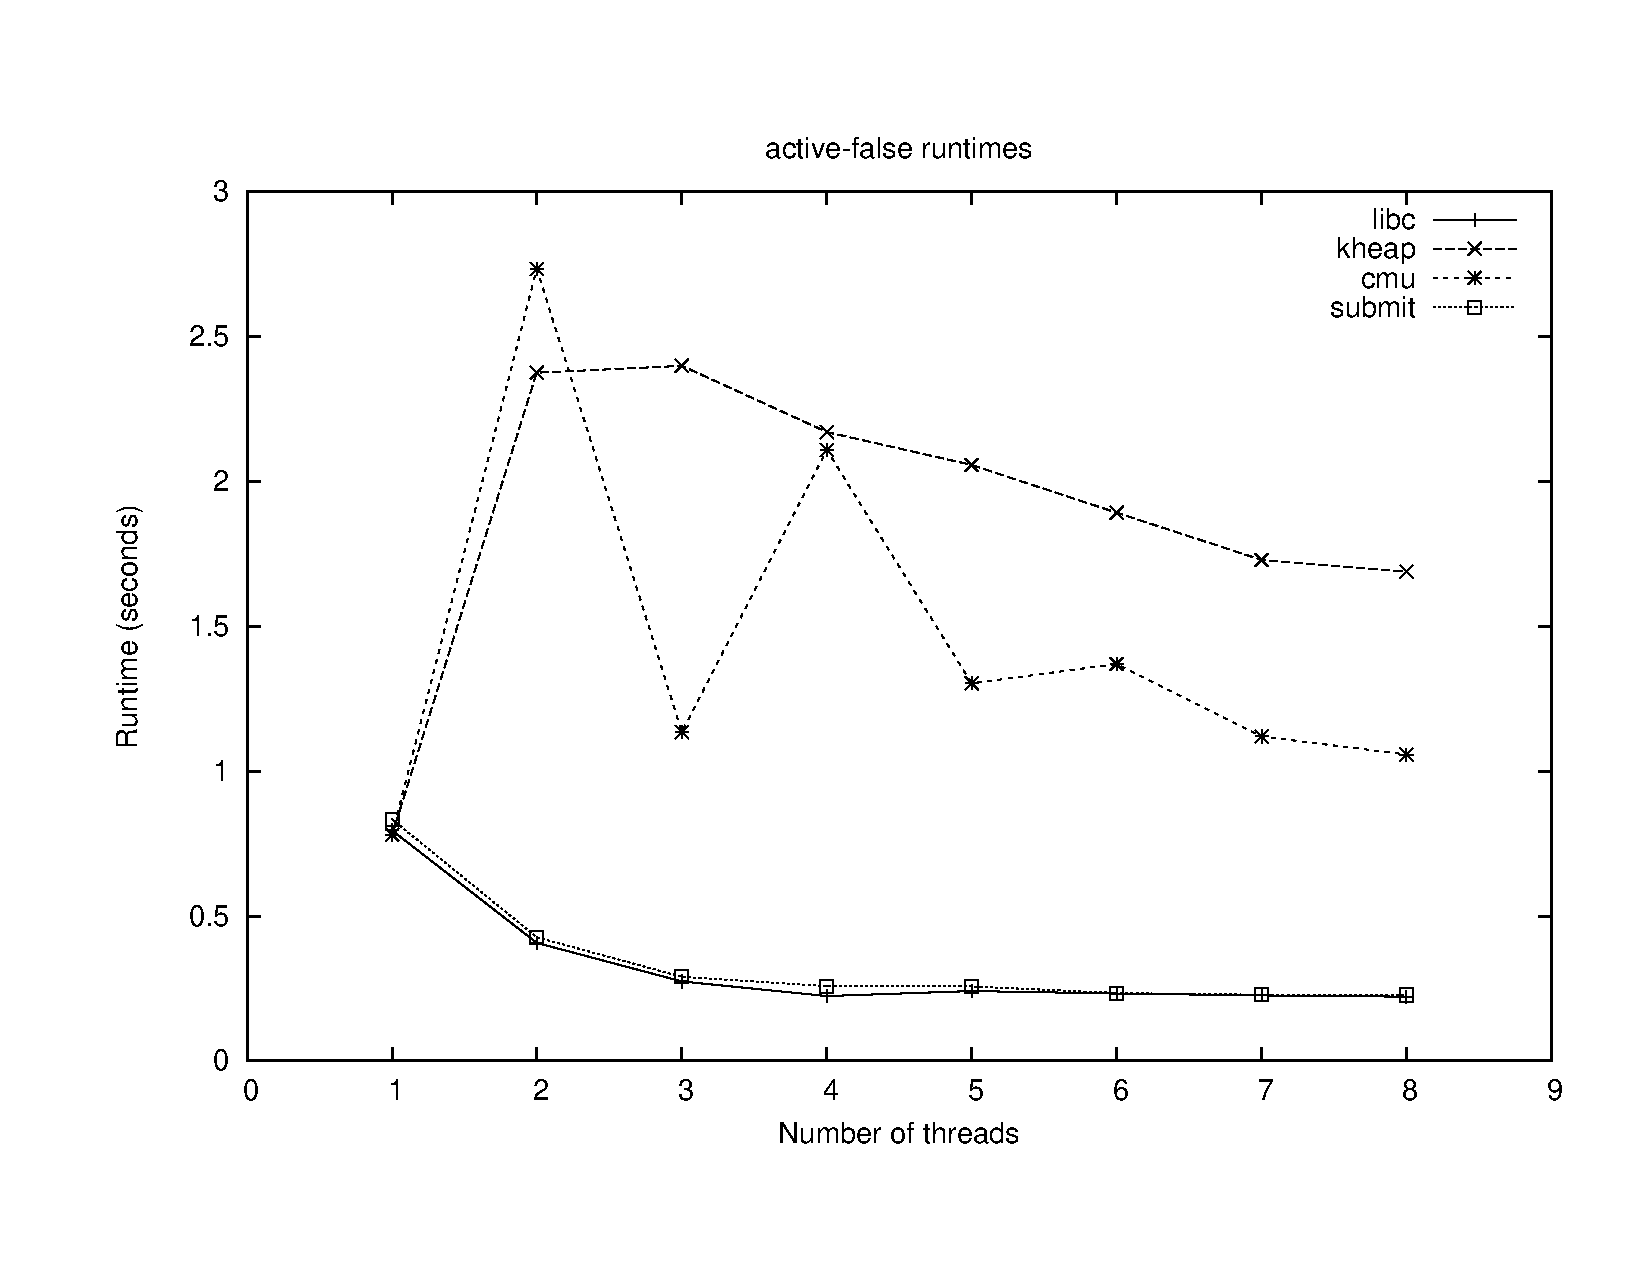
\includegraphics[width=10cm]{cache-thrash.pdf}
\caption{Cache-thrash}
\label{cache-thrash}
\end{figure}
\\
\begin{figure}[!p]
\centering
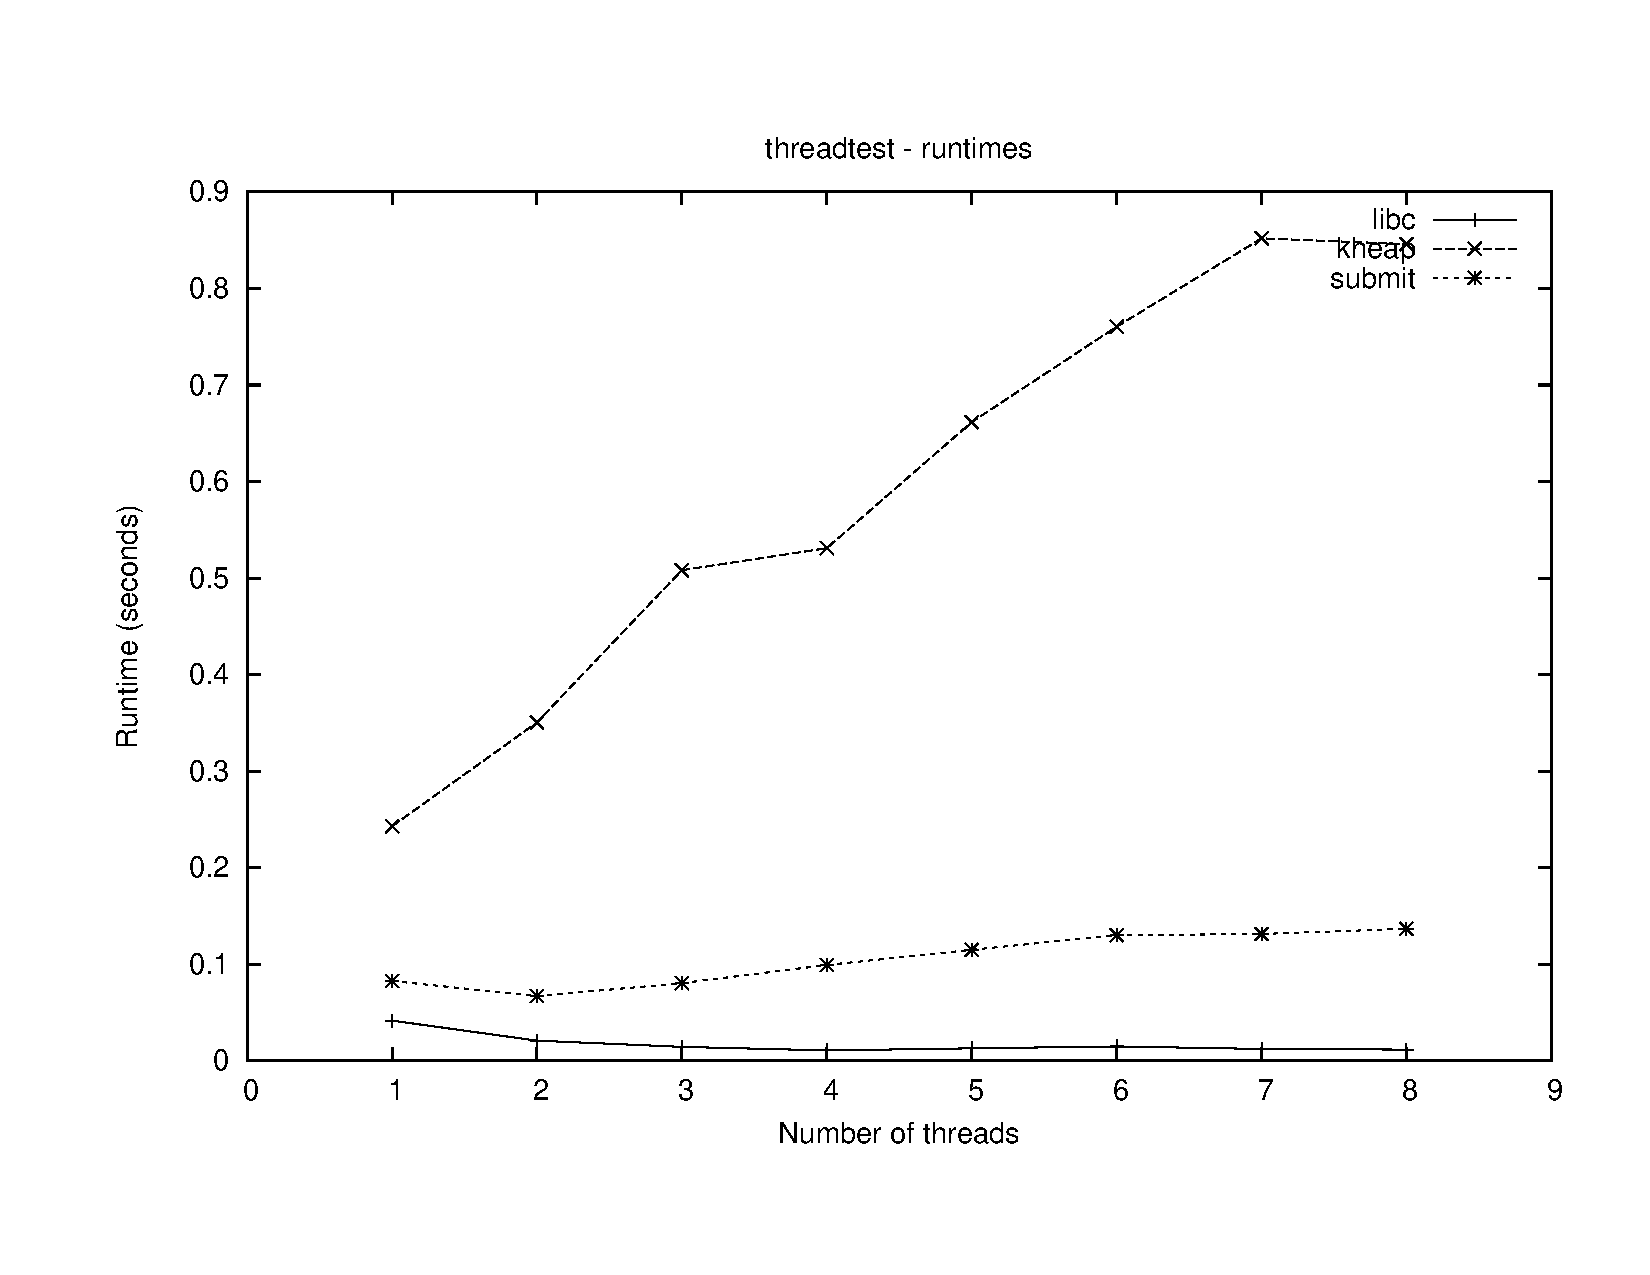
\includegraphics[width=10cm]{threadtest.pdf}
\caption{Threadtest}
\label{Threadtest}
\end{figure}
\\
\newpage
\noindent
\textbf{Scalability}
\\
\section{Discussion}
 
%----------------------------------------------------------------------------------------
%	SECTION 2
%----------------------------------------------------------------------------------------

\newpage
\noindent
%----------------------------------------------------------------------------------------
%	BIBLIOGRAPHY
%----------------------------------------------------------------------------------------
\section{References}
\bibliographystyle{unsrt}
Berger, Emery. "Hoard: A Scalable Memory Allocator for Multithreaded Applications." UMass CS | School of Computer Science. 2000. Web. 11 Nov. 2013. <http://people.cs.umass.edu/>.
\bibliography{sample}
\\
\\
Berger, Emery. "Hoard: A Fast, Scalable, and Memory-Efficient Allocator for Shared-Memory Multiprocessors." cs.utexas.edu. N.p., n.d. Web. <ftp://ftp.cs.utexas.edu/pub/techreports/tr99-22.pdf>.

%----------------------------------------------------------------------------------------


\end{document}
